% !TeX spellcheck = fr_FR
\chapter{Chapitre 4 : Résultats}

Ce chapitre se porte sur les différents essais qui ont été effectués et les résultats de ceux-ci.
Le projet ayant été adapté en cours de route, les sous-chapitres sont organisés de manière chronologique.

\section{Pe Extractor}
La première étape du projet a été de maîtriser et formatter les données du premier simulateur "pe\_extractor".
Comme évoqué lors du chapitre précédent, la génération des bacs contenant la vérité des photons détectés
a une fréquence plus élevée que celle du signal.
J'ai donc regrouper les différents bacs générés sur la même période que le signal :

\begin{lstlisting}[language=iPython,caption={Regroupement des bacs de photons insérés, signal\_sense.ipynb},captionpos=b]
# generator variables
n_sample = 200000
n_sample_init = 0
batch_size = 1
shift_proba_bin = 30
sigma_smooth_pe_ns = 0
bin_size_ns = 0.20
sampling_rate_mhz = 1000 #200 MHz is the sampling rate of Terzina
				#1000 LST + MST
pe_rate_mhz = 150 # 1 to 150 MHz
noise_lsb=4. # 3.5 to 5.5
amplitude_gain=16.
relative_gain_std=0.05

# computed variables
sampling_period_s = 1 / (sampling_rate_mhz * 1e6)
bin_per_sample = ceil(((sampling_period_s) * 1e9) / bin_size_ns)

# parameters omitted for brevity
gen = generator_nsb(...)
data = next(gen)

# data contains in index 0 the configurable batches of the discrete signal
# and in index 1 the batches of truth
# here we configured only 1 batch, which explains the [1][0]
summed_bins = np.sum(data[1][0].reshape(-1, bin_per_sample), axis=1)
\end{lstlisting}

\newpage
Ce qui nous donne le couple de données suivante :
\begin{figure}[tbph!]
	\centering
	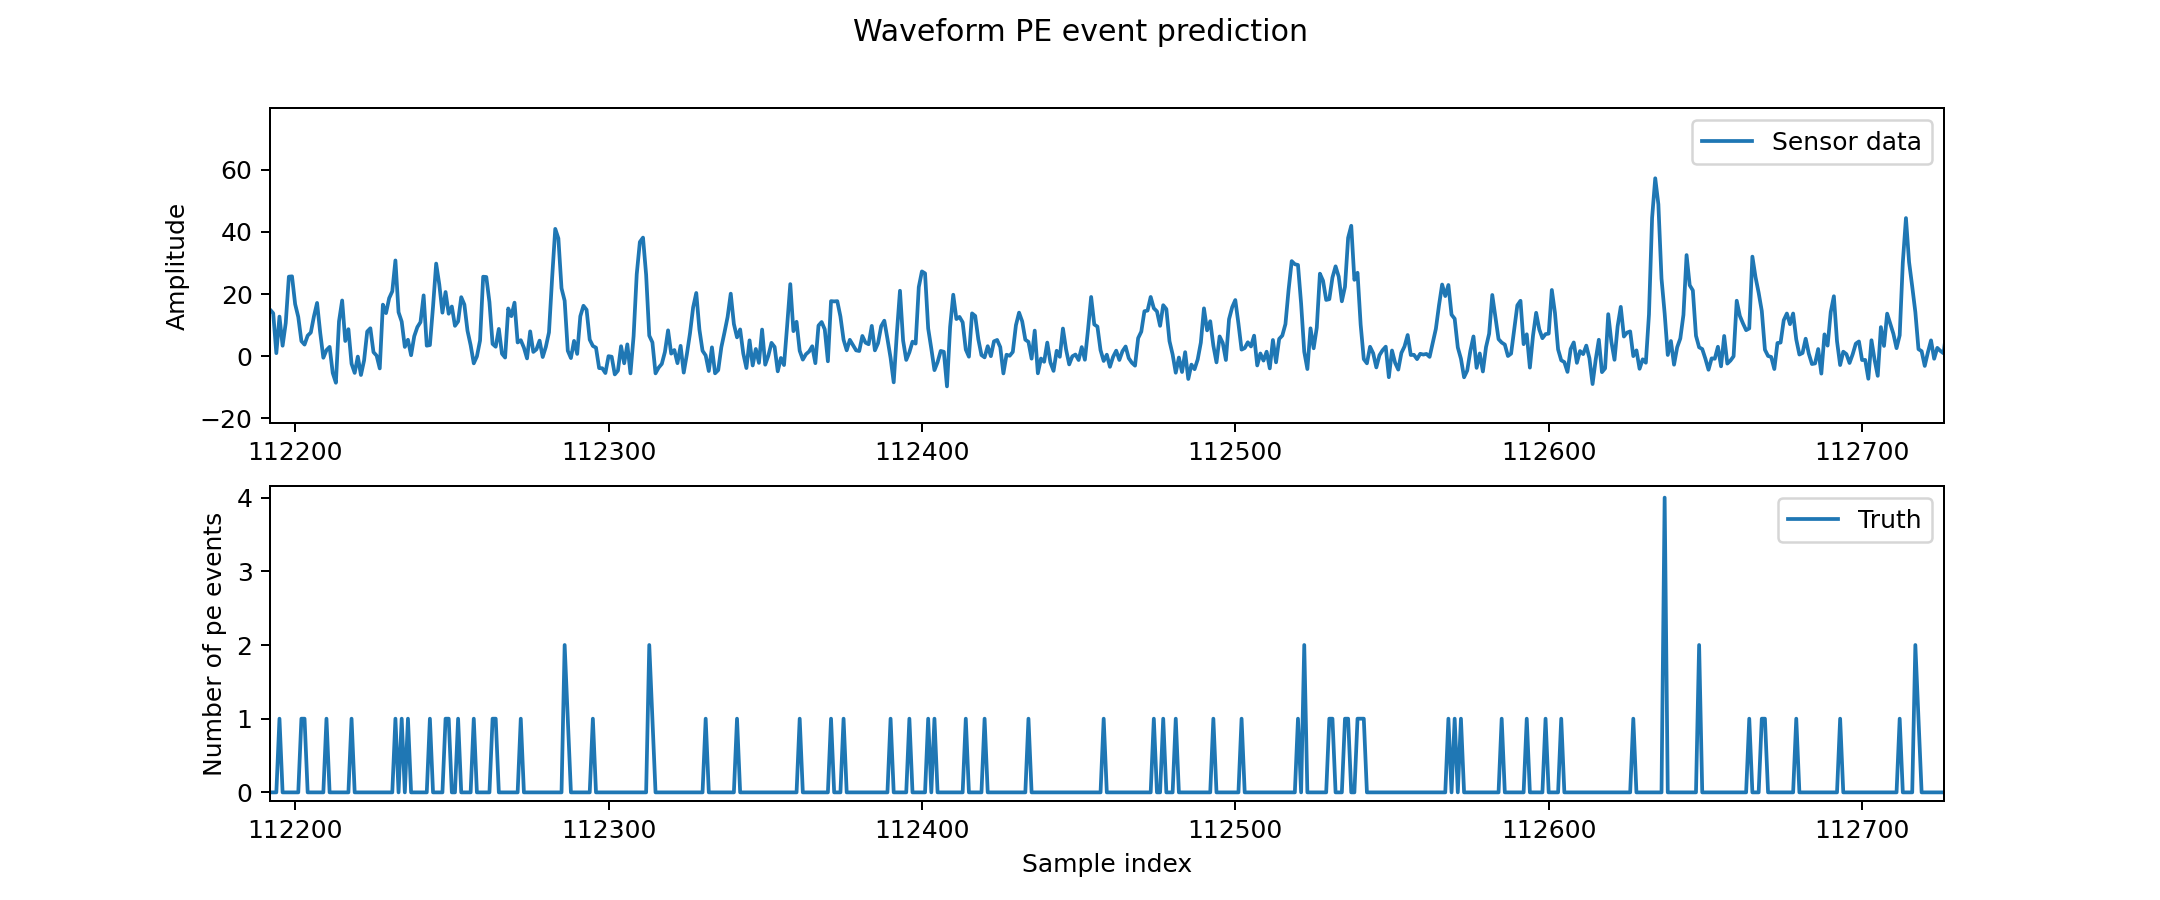
\includegraphics[width=\linewidth]{PeExtractorDataAndTruth.png}
	\caption[Exemple de données générées par "pe\_extractor"]{Exemple de données générées par "pe\_extractor".}
\end{figure}

Les configurations des paramètres du générateur sont restés majoritairement les mêmes au cours du projet 
sauf ceux commentés qui ont évolués au cours du projet dépendant du télescope visé. Il en va de même pour le ficher
d'impulsion correspondant au télescope.

\newpage
\subsection{Création du dataset}
Jusqu'à présent nous n'avons qu'un signal de $200'000$ échantillons. Dans notre cas, il faut un dataset libellé pour commencer 
à entraîner un réseau de neurones. Pour cela, on peut utiliser une technique connue appelée "sliding window" ou fenêtre coulissante en français.
Le nom de cette technique est très descriptif, car c'est comme si l'on regardait nos données à travers une fenêtre qui que l'on déplace du début à la fin celles-ci :

\begin{figure}[tbph!]
	\centering
	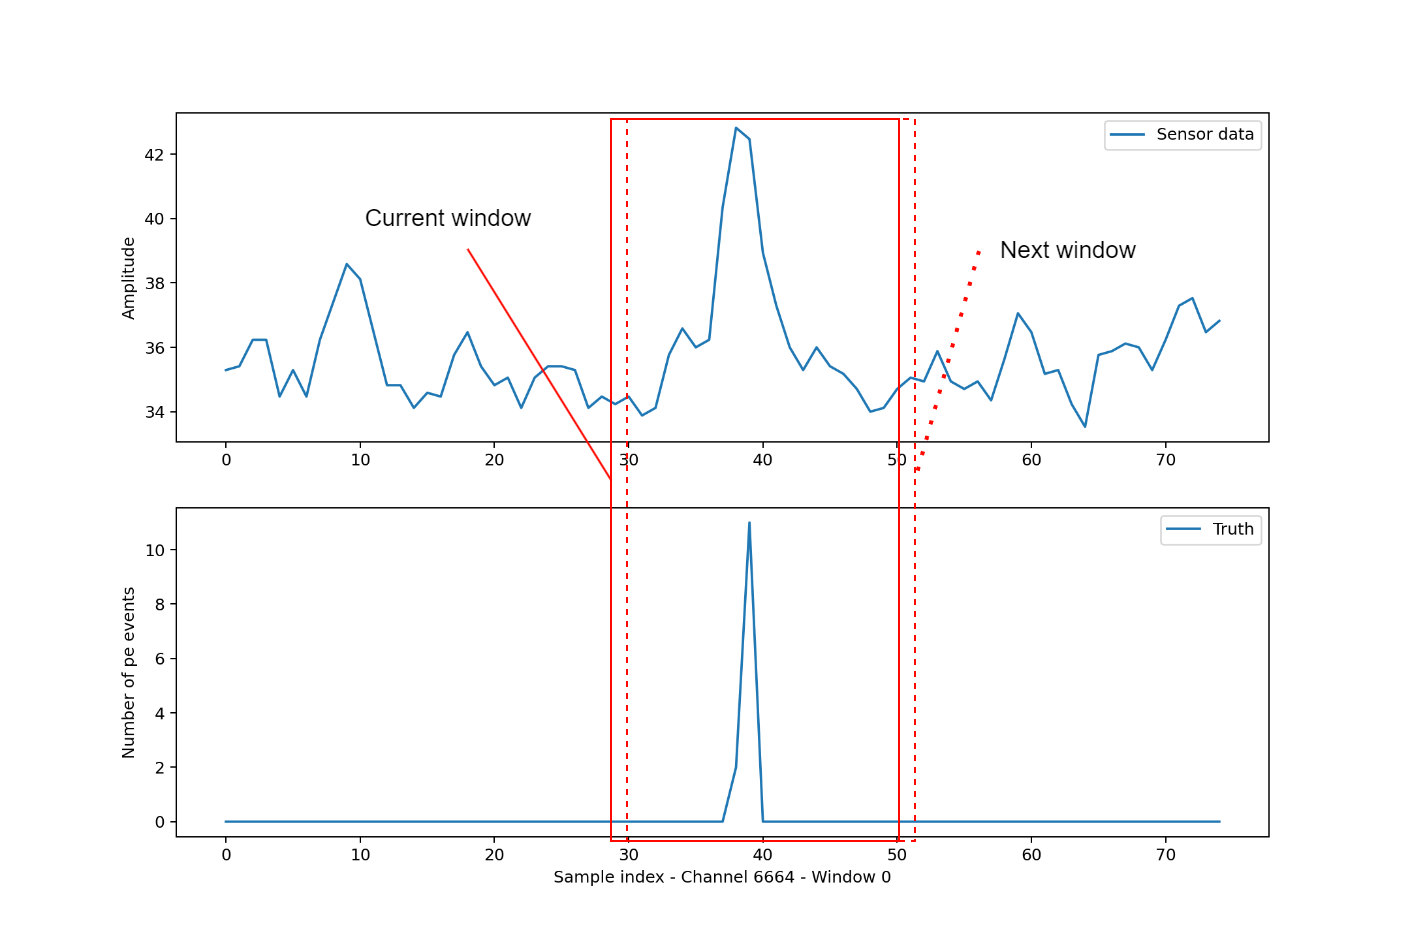
\includegraphics[width=\linewidth]{Sliding window.drawio.png}
	\caption[Exemple de séparation des données par fenêtre coulissante]{Exemple de séparation des données par fenêtre coulissante.}
\end{figure}

Cette technique existant déjà, j'ai utilisé la fonction de la librairie Numpy qui effectue cette transformation.
La seule précaution effectuée a été de bien garder le signal et la vérité dans le même ordre.

Le fonctionnement attendu du réseau de neurones à cet instant était de fonctionner en temps réel juste après les \gls{asic} à bord de Terzina.
Il était donc prévu de garder le modèle le plus petit possible en limitant le nombre d'entrées utilisées. 

Au début des tests, plusieurs configuration de taille de fenêtres ont été testées, 7, 11, 21 jusqu'à un maximum de 51. 
Ces chiffres ont été choisis de manière manuelle dans ce qui avait l'air acceptable pour résoudre ce problème. 
De plus, la conception des des \gls{asic} prévoyait de ne numériser qu'environ une vingtaine d'échantillons lors d'un déclenchement.
Ces différentes tailles de fenêtres n'ont jamais tellement affectés les résultats. Ce qui a été observé est que du moment 
qu'un pic était contenu entièrement dans les valeurs d'entrées les modèle semblait avoir assez de données pour le détecter.

\section{Premiers tests}

\subsection{Détection booléenne de photon-électron}
Au tout début du projet, j'ai essayé de simplement détecter la présence ou non d'au moins un \gls{pe} exactement au centre de chaque fenêtre générée.

Pour cela, j'ai mis en place un réseau neuronal convolutif de classification simple.
Le résultat attendu de ce réseau est une seule estimation de la présence ou non d'un photon à l'échantillon central.
\begin{figure}[tbph!]
	\centering
	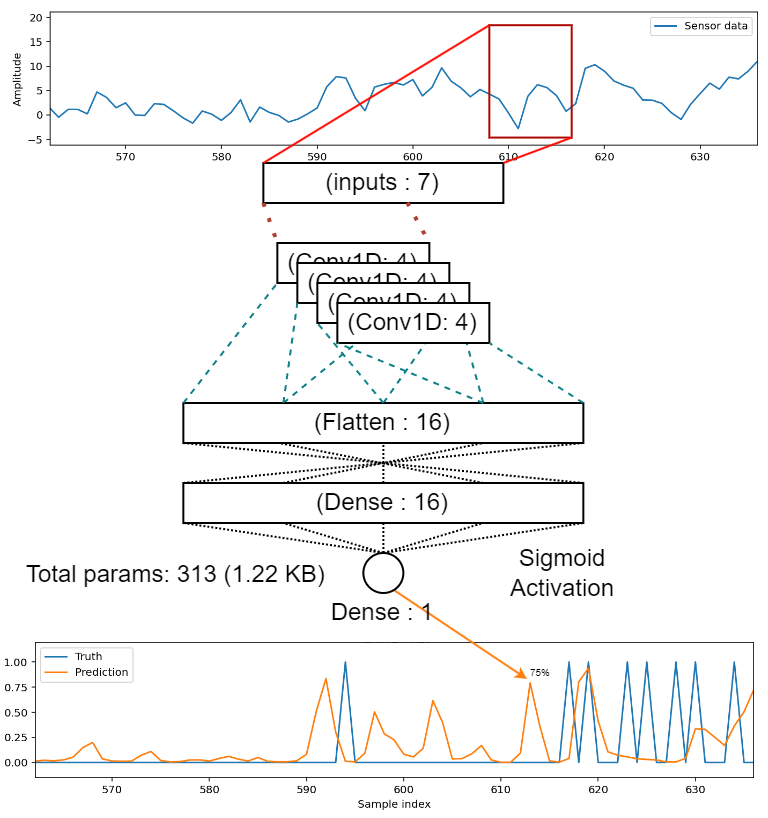
\includegraphics[width=0.6\linewidth]{cnn_simple.drawio.png}
	\caption[Diagramme de fonctionnement du premier CNN simple]{Diagramme de fonctionnement du premier CNN simple.}
\end{figure}

Les résultats observés de cette architecture n'étaient pas bons.
Cela pour plusieurs raisons, le premier étant l'un des pièges les plus courant des réseaux neuronaux : des données erronées.
Cette première erreur provenait de transformation des bacs en résultat booléen utilisé dans cette phase d'entraînement.
Lors de cette transformation, l'échantillon testé pour la présence d'un \gls{pe} s'est avéré être le premier de la fenêtre.

Cette première expérience m'a poussé à développer des vues au "cas par cas" où chaque inférence du modèle peut être examinée en détails.
Cette vue affiche les données d'entrée, la vérité attendue et le résultat du modèle ce qui permet de visualiser son comportement après entraînement. 

Cependant, même après avoir corrigé le dataset d'entraînement, les résultats, bien que légèrement améliorés, restaient non fiables à cause de beaucoup de
faux positif et faux négatifs.

\subsection{Estimation calorimétrique de photon-électron par régression}
Pour permettre de au lieu d'entraîner le modèle sur une seule vérité au centre de la fenêtre analysée, ce serait sur chaque 
échantillon que le réseau neuronal donnera une estimation de la présence ou non d'un \gls{pe}.

Ce nouveau modèle a immédiatement mieux performé que le précédant :

\begin{figure}[tbph!]
	\centering
	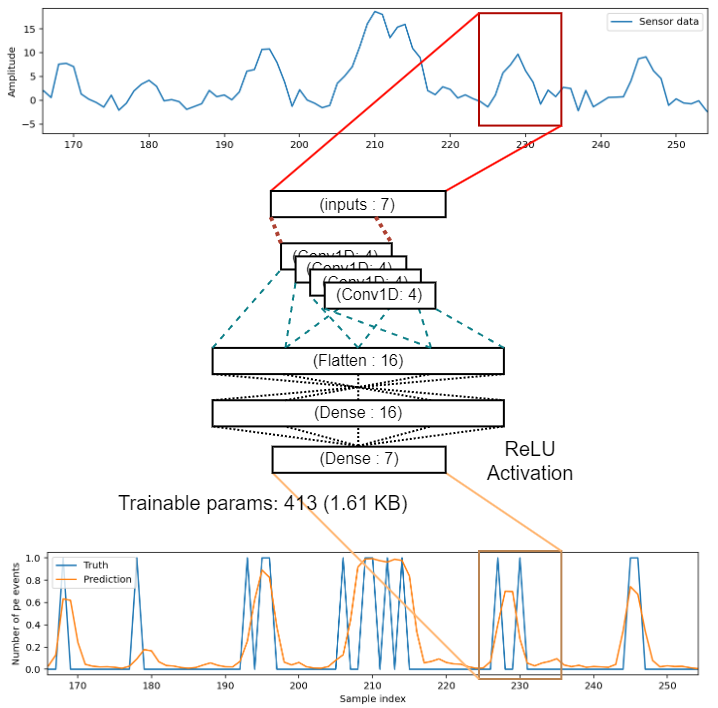
\includegraphics[width=0.6\linewidth]{cnn_mult.drawio.png}
	\caption[Diagramme de fonctionnement du deuxième CNN à multiple sortie]{Diagramme de fonctionnement du deuxième CNN à multiple sortie.}
\end{figure}

En modifiant les différents paramètres de chaque couche, il est aussi possible d'améliorer les performances de celui-ci.
De plus, en ne calculant plus la présence de manière booléenne mais en estimant la quantité de \gls{pe} présents 
en changeant la fonction d'activation finale pour utiliser la fonction mathématique "ReLU" qui n'est pas confinée 
à l'intervalle $ \left[ 0, 1\right] $ comme la sigmoïde mais à $ \left[0, +\infty\right[ $, il est possible d'entraîner le modèle
pour qu'il estime le nombre de \gls{pe} à un instant $t$ dans une fenêtre. 

%TODO comparaisons qui soient bien justifiées et qui soient dans le même pipeline et données

% \subsection{Réseau de neurones convolutif}
% Dans le cadre de Terzina, c'est l'approche que nous avons privilégiée de par sa simplicité et le peu de resources qu'elle utilise.


\subsection{Fichiers de simulation Corsika}

Pour utiliser ces fichiers de simulations, il a d'abord fallu recréer les signaux avec l'outil qui m'avait été fourni par l'\gls{unige} : "pyeventio\_example".
Sur le cluster Yggdrasil, j'ai compilé et utilisé l'exécutable "runana" de manière distribuée grace à un script bash :

\begin{lstlisting}[language=iBash,caption={Script de génération des signaux à partir de fichier de simulation, data/slurm-run.sh},captionpos=b]
#!/bin/sh

# manage cluster modules
module purge
module load GCC/11.2.0  OpenMPI/4.1.1 ROOT/6.24.06

# select events range to generate
ev_start=0
ev_stop=1000

# select the simulation file
inRootFiles="/srv/beegfs/scratch/shares/heller/Leonid/mono-lst-sipm-pmma-3ns-v1_triggerless/gamma/0000/corsika_0000ID.root"
rndseed="1312312"

for ((evID=ev_start; evID<=ev_stop; evID++))
do
	# location of output file
	binFileOut="/home/users/p/perrinya/scratch/bin_data/gamma_ev"$evID"_out.bin"
	# recreate complete waveform with truths
	srun --time "00:00:30" /home/users/p/perrinya/pyeventio_example/runana 333 "$inRootFiles" "$evID" "$binFileOut" "$rndseed" &
done
\end{lstlisting}

Les fichiers binaires produits utilisent beaucoup plus de place que les fichiers ROOT. Par exemple, le fichier "corsika\_0000ID.root" comportant les
informations nécessaires à reconstruire environ $500'000$ pluies Cherenkov, d'une durée d'environ $75ns$ chacune, ne pèse que $1.2GB$.
En comparaison, les fichier binaires prennent plus de $2.38GB$ pour seulement 1000 évènements. 
La totalité des signaux brutes du fichier prendrait une taille de : $500'000/1000 * 2.38GB = 1.19TB$

Cependant, ces fichiers binaires ne sont que la première étape pour créer un jeu de données utilisable par nos réseaux de neurones.
Ceux-ci sont structurés de la manière suivante :

\begin{figure}[tbph!]
	\centering
	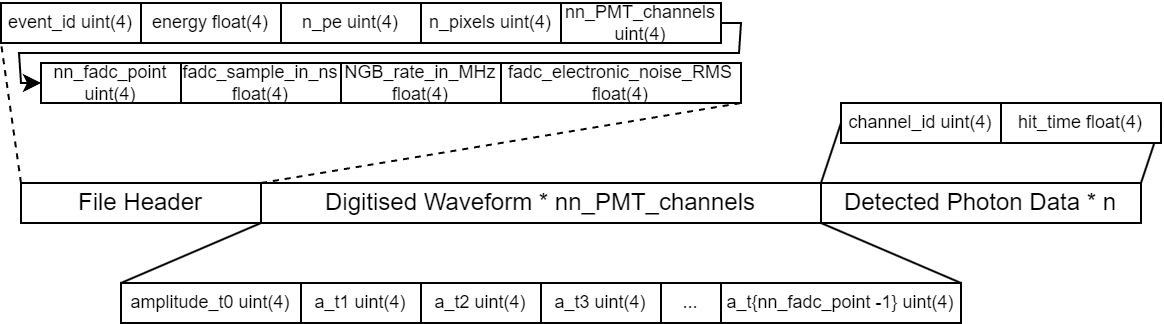
\includegraphics[width=\linewidth]{Pyeventio_binary_file_content.drawio.png}
	\caption[Structure des fichiers binaires de simulations]{Structure des fichiers binaires de simulations.}
\end{figure}

J'ai donc du créer un lecteur capable de parser ces fichiers binaires et de recréer une vérité sur la même fréquence que le signal d'entrée.
Pour cela, la lecture du header et du signal ce fait simplement en lisant et stockant des variables dans des tableaux en mémoire.
Cependant quelques calculs et vérifications doivent être faites pour les photons détectés par la caméra. 
En premier, il faut convertir l'instant de l'impact en numéro d'échantillon en divisant par la période d'acquisition.
Puis il faut vérifier si ce photon a bien été capturé pendant la durée du signal, car ceux-ci peuvent avoir été détectés
avant ou après, ceci probablement dû à la gestion de la simulation.

\newpage
Au final on se retrouve avec des données similaires au premier simulateur :
\begin{figure}[tbph!]
	\centering
	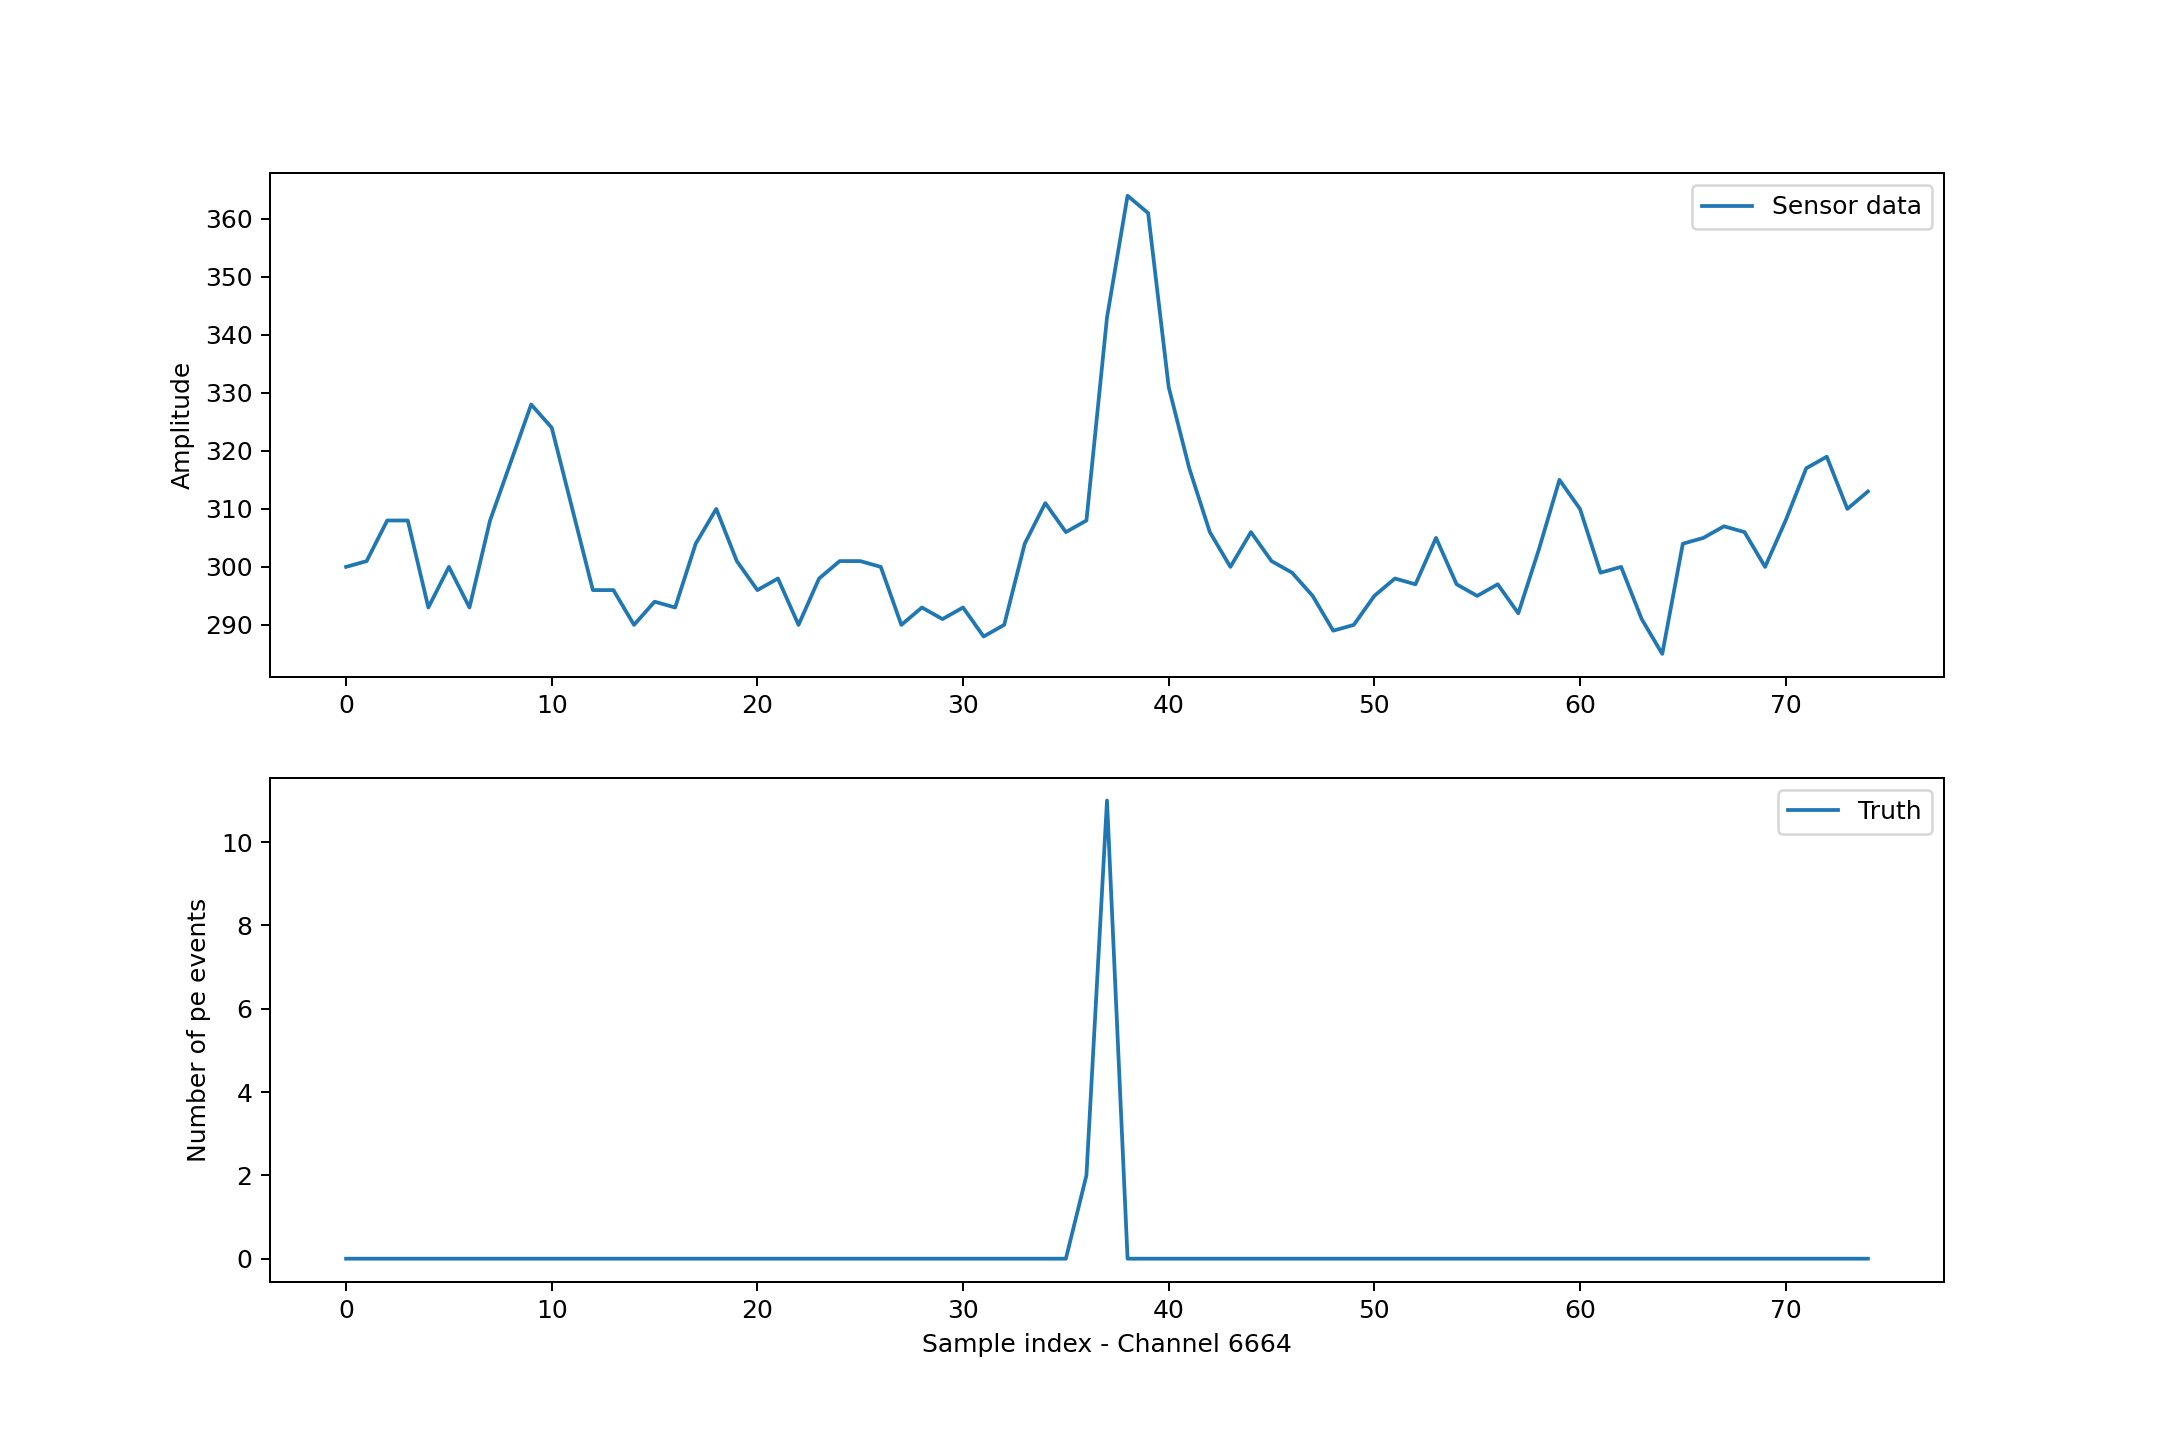
\includegraphics[width=\linewidth]{BinaryRecomposedSignalTruth.png}
	\caption[Exemple de données générées par simulations Corsika]{Exemple de données générées par simulations Corsika.}
\end{figure}

Cependant, même dans cet état, les données ne sont pas encore utilisables. Lorsque l'on regarde l'amplitude 
du signal contenu dans ces fichiers binaires, ceux-ci sont encodés sur des entiers. Pour réduire ces valeurs avant d'essayer
d'entraîner des réseaux neuronaux, il m'a été conseillé de normaliser ces données en les divisant par 8,5 en rapport avec les
capteurs simulés.

De plus, nous avons découvert que les temps d'impacts des photons détectés étaient un peu en avance par rapport
au signal. Nous avons donc ajouté un délai de 2 échantillons lors du parsing du fichier, pour que les pics de vérité arrivent en 
même temps ou avec un léger retard pour que le réseau de neurones puisse utiliser les échantillons précédents comme information utile.

\newpage
\begin{figure}[tbph!]
	\centering
	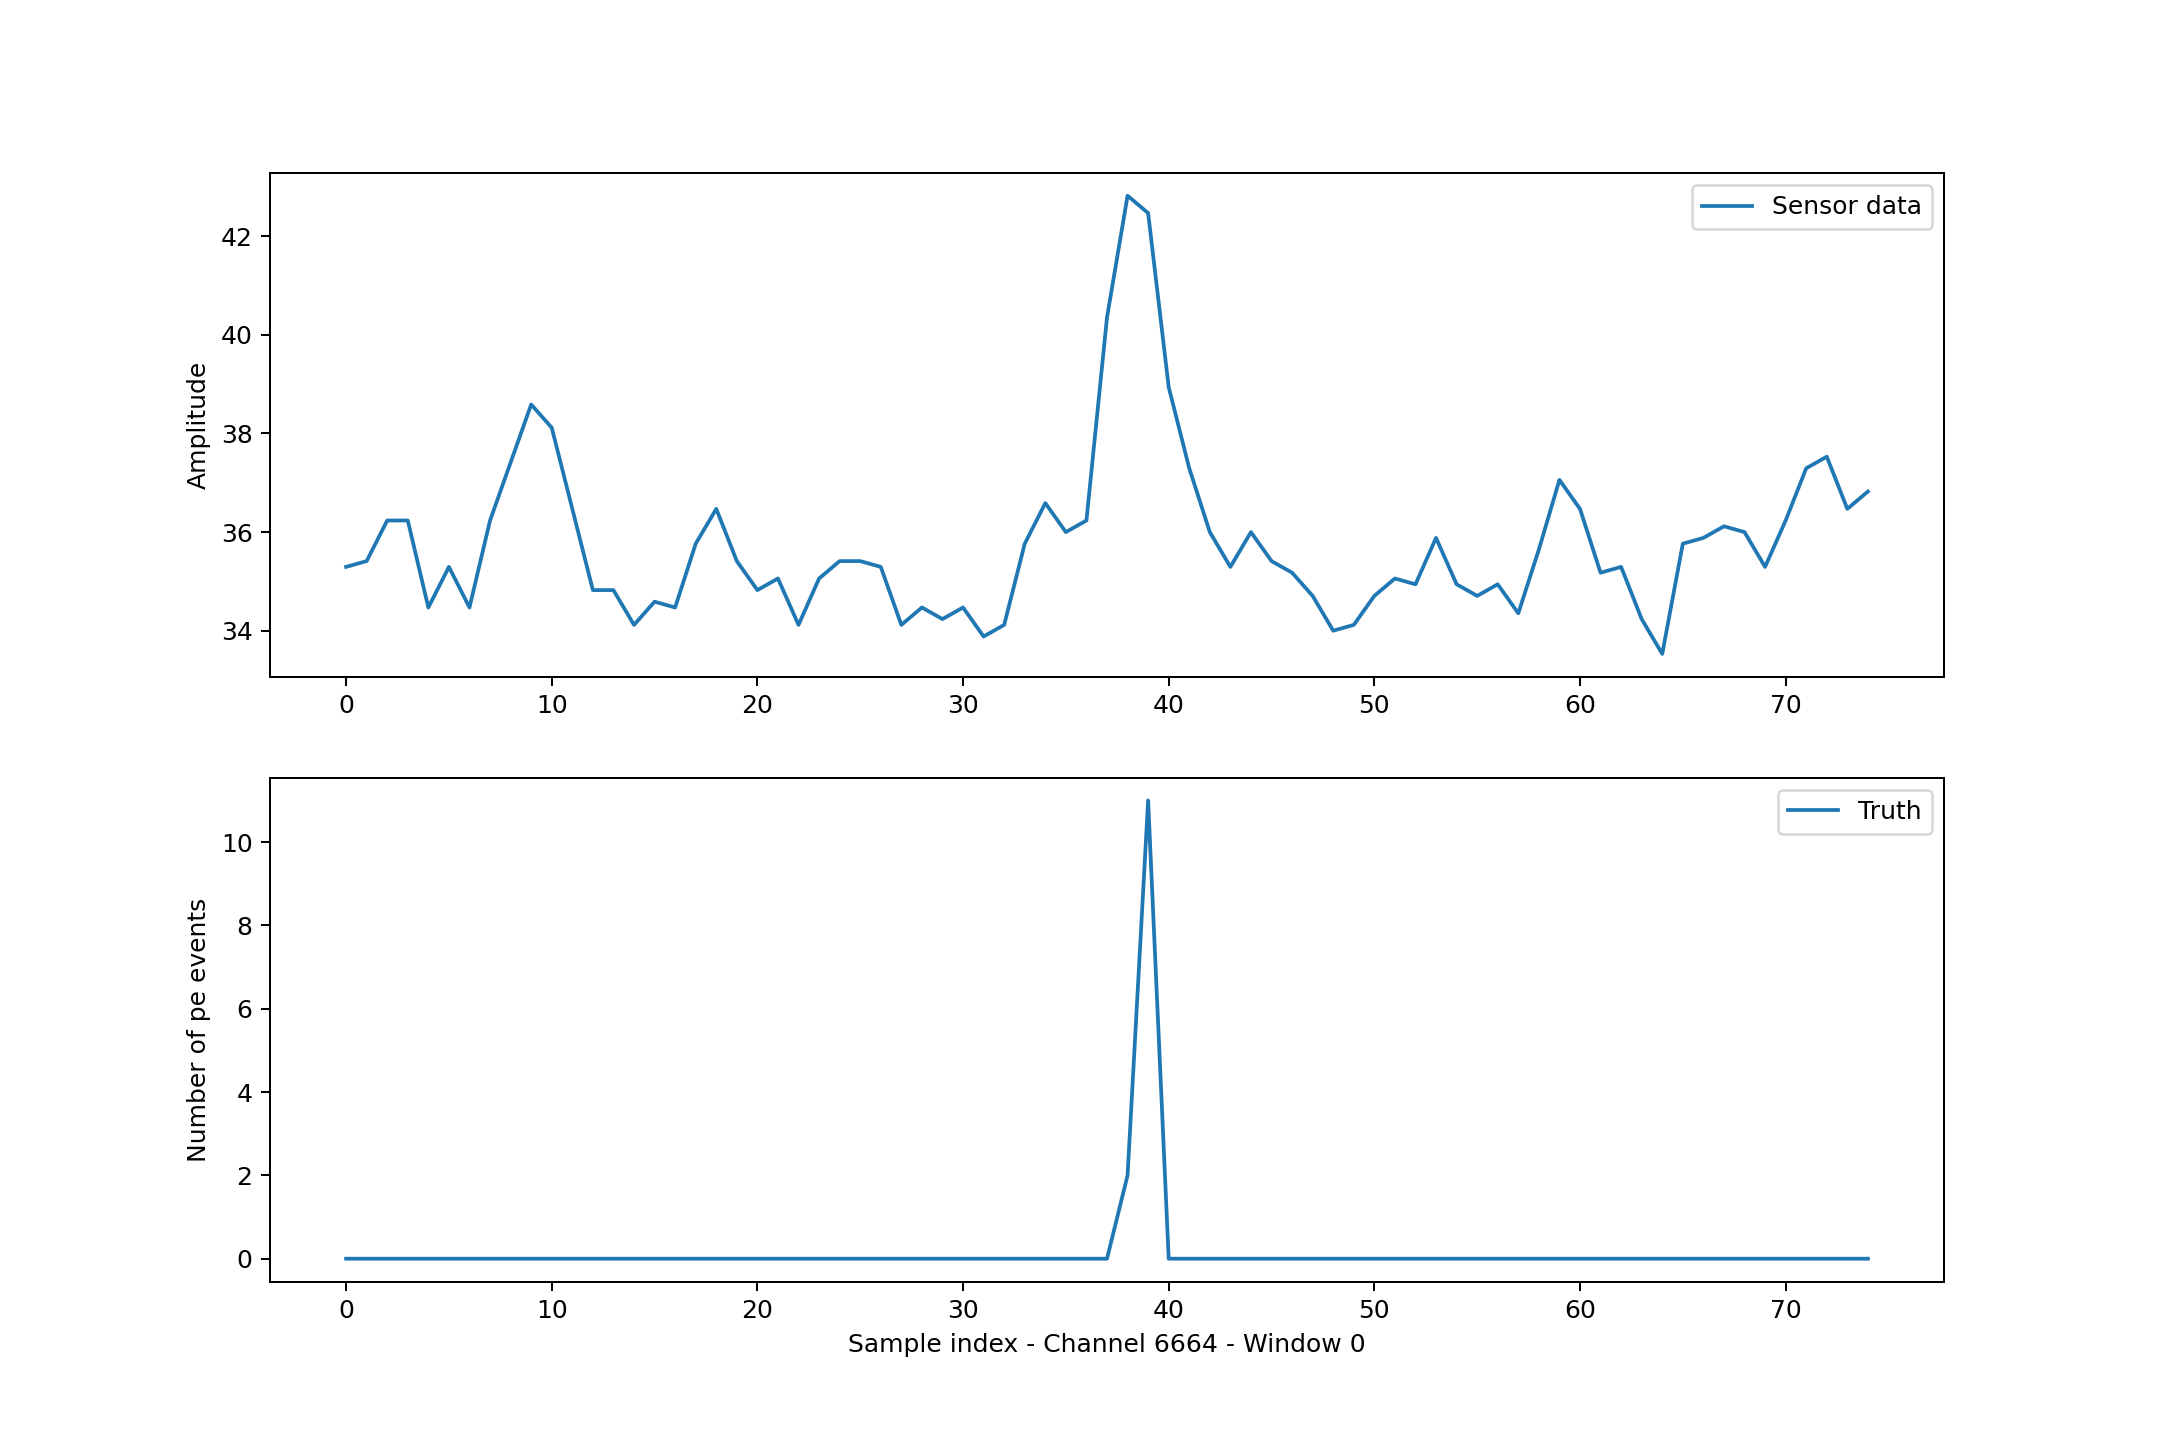
\includegraphics[width=\linewidth]{BinaryRecomposedSignalTruthNormalized.png}
	\caption[Données Corsika normalisées]{Données Corsika normalisées.}
\end{figure}












\subsection{Création de dataset}
C'est pendant cette même étape de séparation que l'on peut facilement effectuer deux autres actions pour améliorer notre dataset.

La première action, est de séparer nos données en deux. La première partie sera utilisée pour entraîner le réseau tandis que la deuxième ne
lui sera jamais montré lors de l'entraînement mais seulement lors d'une étape de validation. Cela dans l'optique d'éviter l'overfitting
et valider que le modèle puisse fonctionner sur des données qu'il n'a jamais vu auparavant.

La deuxième action consiste à mélanger le dataset pour éviter de s'entraîner avec des données dans l'ordre, pour pousser 
le modèle à trouver des motifs dans les données mêmes.

\subsection{Corsika répartition du dataset}
Spécifiquement dans le cas des données Corsika, il s'est rapidement avéré que la répartition des \gls{pe} dans le dataset était problématique.
Cela paraît logique
